\en{The Chudnovsky formula for calculating $\pi$ reads}%
\de{Die Chudnovsky-Formel zur Berechnung von $\pi$ lautet}
%\vspace*{0.3cm}
$$\frac{1}{\pi} = 12\cdot\sum_{n=0}^\infty \frac{(-1)^n(6n)!}{(3n)!(n!)^3}\cdot \frac{13591409 + 545140134 n}{ 640320^{3n+3/2}}.$$
%\vspace*{0.3cm}


\en{It is particularly \emph{efficient}, because it yields on average $14\ko1816$ decimal digits of $\pi$ per iteration (see Thm.~\ref{\en{EN}14dezi}). That's why it is being used in most world record computations since 1989\footnote{The Chudnovsky algorithm develops its full speed only when the summation is done with "binary splitting" and a fast multiplication like Schönhage Strassen is implemented. Under these conditions, the time for computing $n$ digits of $\pi$ with the Chudnovsky algorithm is $O(M(n)\log^2(n))$, where $M(n)=O(n\log(n)\log(\log(n)))$ is the time for $n$-digit multiplication.}. For an overview about these world records see \cite{\en{EN}agar}, \cite{\en{EN}ycru} or Fig.~\ref{\en{EN}fighist}.}%
\de{Sie ist besonders \emph{effizient}, weil sie pro Summand durchschnittlich $14\ko1816$ weitere Dezimalen liefert (siehe dazu auch Thm.~\ref{\en{EN}14dezi}). Deshalb wird sie seit 1989 für die meisten $\pi$-Berechnungs-Weltrekorde verwendet\footnote{Die volle Geschwindigkeit entwickelt der Chudnovsky-Algorithmus erst, wenn man für die Summation \glqq binary splitting\grqq~verwendet und eine schnelle Multiplikation wie Schönhage-Strassen. Dann braucht man zur Berechnung von $n$ Dezimalen nur $O(M(n)\log^2(n))$ Zeit, wobei $M(n)=O(n\log(n)\log(\log(n)))$ die Zeit für eine $n$-stellige Multiplikation ist.}. Für einen Überblick über diese Weltrekorde siehe \cite{\en{EN}agar}, \cite{\en{EN}ycru} oder Abb.~\ref{\en{EN}fighist}.}

\en{Moreover, it is particularly \emph{beautiful}, because its coefficients are such huge natural numbers.
If you only want to know where these coefficients come from, you can read \cite{\en{EN}Milla2021}, which is much shorter (7 pages) but also more advanced.}%
\de{Außerdem ist sie besonders \emph{schön}, weil die Koeffizienten riesige natürliche Zahlen sind. Wer direkt wissen will, woher die Koeffizienten kommen, kann auch \cite{\en{EN}Milla2021} lesen, was viel kürzer ist (7 Seiten) aber natürlich mehr Kenntnisse voraussetzt.}%

\begin{figure}[h!]
\centering
\pgfkeys{/pgf/number format/.cd,1000 sep={}}
\pgfplotsset{every axis legend/.style={
cells={anchor=center},% Centered entries
inner xsep=3pt,inner ysep=2pt,nodes={inner sep=2pt,text depth=0.15em},
anchor=north west,
shape=rectangle,
fill=none,
%draw=none,
%at={(rel axis cs:0.04,0.88)}
at={(rel axis cs:0.4,0.3)}
}
}
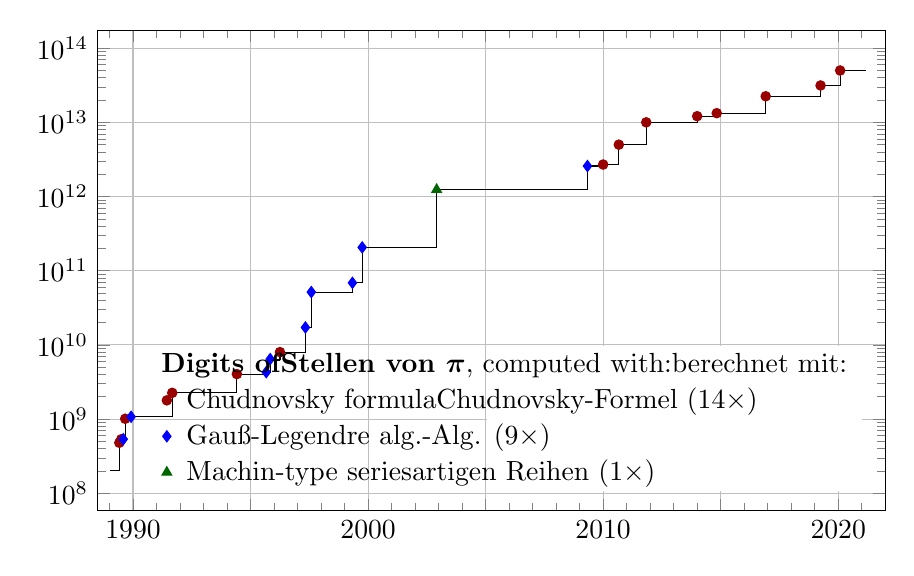
\begin{tikzpicture}
\begin{semilogyaxis}[scale only axis=true,
  width=10cm, height=6.1cm,
  %width=9.2cm, height=\en{3.65cm}\de{3.35cm},
  legend cell align={left},
  minor x tick num=4,
  %xtick={1990,2000,2010,2020},
  %minor tick length = 6pt,
 % xtick={1990,1991,2000,2001,2010,2011,2020,2021},
  %xtick={1990,2000,2010,2020},
  minor xtick={1989,1991,1992,1993,1994,1995,1996,1997,1998,1999,
                    2001,2002,2003,2004,2005,2006,2007,2008,2009,
                    2011,2012,2013,2014,2015,2016,2017,2018,2019,2021},
  xticklabels={,,1990,,2000,,2010,,2020,},
  grid=major, 
    major grid style=gray!50,
  ytick={1e8,1e9,1e10,1e11,1e12,1e13,1e14},
  xmin=1988.5,
  xmax=2022,
  yticklabel pos=left,
  %x tick label as interval,
  %ylabel=\en{decimal digits of}\de{Dezimalen von} $\pi$,
legend pos = south east]%,xlabel=\en{year}\de{Jahr}]
\addlegendimage{empty legend}\addlegendentry{\hspace{-.2cm}\textbf{\en{Digits of}\de{Stellen von} \boldmath{$\pi$}}, \en{computed with:}\de{berechnet mit:}}
%\addplot[only marks, mark size=0pt] coordinates { (1999.666667, 1011196691) };
%\addplot[only marks, mark size=0pt] coordinates { (1999.666667, 1011196691) };
%\addplot[only marks, mark size=0pt] coordinates { (1999.666667, 1011196691) };
\addplot[only marks, mark=*, mark size=1.7pt, red!60!black] coordinates {
(1989.416667, 480000000) % Chudnovsky brothers (Chud)
(1989.500000, 535339270) % Chudnovsky brothers (Chud)
(1989.666667, 1011196691) % Chudnovsky brothers (Chud)
(1991.666667, 2260000000) % Chudnovsky brothers (Chud)
(1994.416667, 4044000000) % Chudnovsky brothers (Chud)
(1996.250000, 8000000000) % Chudnovsky brothers (Chud)
(2010.000000, 2699999990000) % Fabrice Bellard (Chud)
(2010.666667, 5000000000000) % Shigeru Kondo & Alex Yee (Chud)
(2011.833333, 10000000000050) % Shigeru Kondo (Chud)
(2014.000000, 12100000000050) % Shigeru Kondo (Chud)
(2014.833333, 13300000000000) % Sandon van Ness (Chud)
(2016.916667, 22459157718361) % Peter Trueb (Chud)
(2019.250000, 31415926535897) % Emma Haruka Iwao (Chud)
(2020.083333, 50000000000000) % Timothy Mullican (Chud)
};
%\draw [fill=black,black] (1990,2e7) rectangle (1991,10e7);
%\draw [fill=black,black] (1990,10e13) rectangle (1991,2e14);
%\draw [fill=black,black] (2000,2e7) rectangle (2001,10e7);
%\draw [fill=black,black] (2000,10e13) rectangle (2001,2e14);
%\draw [fill=black,black] (2010,2e7) rectangle (2011,10e7);
%\draw [fill=black,black] (2010,10e13) rectangle (2011,2e14);
%\draw [fill=black,black] (2020,2e7) rectangle (2021,10e7);
%\draw [fill=black,black] (2020,10e13) rectangle (2021,2e14);
\draw [fill=white,white] (2005.1,1.1e8) rectangle (2021,0.95e10);
\addplot[only marks, mark=diamond*, blue] coordinates { 
%(1982, 2097144) % GL2
%(1982, 4194288) % GL2
%(1982, 8388576) % GL2
%(1983, 16777206) % GL2
%(1986.083333, 29360111) % B2. B4
%(1986.75, 33554414) % GL2. B4
%(1986.833333, 67108839) % GL2
%(1987.083333, 134214700) % GL2. B4
%(1988.083333, 201326551) % Kanada et al (GL2, B4)
(1989.583333, 536870898) % Kanada et al (GL2, B4)
(1989.916667, 1073740799) % Kanada et al (GL2)
(1995.666667, 4294960000) % Kanada et al (GL2, B4)
(1995.833333, 6442450000) % Kanada et al (GL2, B4)
(1997.333333, 17179869142) % Kanada et al (GL2, B4)
(1997.583333, 51539600000) % Kanada et al (GL2, B4)
(1999.333333, 68719470000) % Kanada et al (GL2, B4)
(1999.750000, 206158430000) % Kanada et al (GL2, B4)
(2009.333333, 2576980377524) % Daisuke et al (GL2, B4)
};

\addplot[only marks, mark=triangle*, green!40!black] coordinates {
%(1981, 2000036) % arctan
%(1981, 2000050) % ?
(2002.916667, 1241100000000) % Kanada et al (Machin-Type)
};
%\addplot[dotted]  coordinates { (1988.083333, 201326551)(1989.0, 201326551)};
\addplot[solid]  coordinates { 
%(1988.083333, 201326551)
(1989.0, 201326551)
(1989.416667, 201326551) 
(1989.416667, 480000000) 
(1989.500000, 480000000) 
(1989.500000, 535339270) 
(1989.583333, 535339270) 
(1989.583333, 536870898) 
(1989.666667, 536870898) 
(1989.666667, 1011196691)
(1989.916667, 1011196691) 
(1989.916667, 1073740799) 
(1991.666667, 1073740799)
(1991.666667, 2260000000) 
(1994.416667, 2260000000)
(1994.416667, 4044000000) 
(1995.666667, 4044000000)
(1995.666667, 4294960000) 
(1995.833333, 4294960000)
(1995.833333, 6442450000) 
(1996.250000, 6442450000) 
(1996.250000, 8000000000) 
(1997.333333, 8000000000)
(1997.333333, 17179869142)
(1997.583333, 17179869142)
(1997.583333, 51539600000) 
(1999.333333, 51539600000) 
(1999.333333, 68719470000) 
(1999.750000, 68719470000) 
(1999.750000, 206158430000) 
(2002.916667, 206158430000) 
(2002.916667, 1241100000000) 
(2009.333333, 1241100000000)
(2009.333333, 2576980377524) 
(2010.000000, 2576980377524) 
(2010.000000, 2699999990000) 
(2010.666667, 2699999990000) 
(2010.666667, 5000000000000) 
(2011.833333, 5000000000000) 
(2011.833333, 10000000000050)
(2014.000000, 10000000000050) 
(2014.00000, 12100000000050) 
(2014.833333, 12100000000050)
(2014.833333, 13300000000000)
(2016.916667, 13300000000000) 
(2016.916667, 22459157718361) 
(2019.250000, 22459157718361)
(2019.250000, 31415926535897)
(2020.083333, 31415926535897)
(2020.083333, 50000000000000) 
(2021.2, 50000000000000) }; 

%\addplot[only marks, mark=pentagon*, orange!40!black] coordinates {
%(1985.833333, 17526200) % Rama
%};

\addlegendentry{~\en{Chudnovsky formula}\de{Chudnovsky-Formel} (14$\small{\times}$)};
\addlegendentry{~Gauß-Legendre\en{ alg.}\de{-Alg.} (9$\small{\times}$)};
\addlegendentry{~Machin-\en{type series}\de{artigen Reihen} (1$\small{\times}$)};
%\addlegendentry{~\en{Ramanujan's formula}\de{Ramanujan-Formel} (1)}
\end{semilogyaxis}
\end{tikzpicture}\vspace*{-8pt}
\caption{\en{Number of known digits of $\pi$ since 1989}\de{Anzahl bekannter Stellen von $\pi$ seit 1989}}
\label{\en{EN}fighist}
\end{figure}

\en{In this paper, we prove the Chudnovsky formula in detail. We only need a basic knowledge of complex analysis and of analysis -- for example the ratio test, Leibniz's rule, Laurent series, the residue theorem and the Picard-Lindelöf theorem.}%
\de{In diesem Aufsatz beweisen wir die Chudnovsky-Formel ausführlich. Dabei werden nur grundlegende Kenntnisse in Funktionentheorie und Analysis vorausgesetzt, z.B.~Quotientenkriterium, Leibnizregel, Laurentreihen, Residuensatz und der Satz von Picard-Lin\-delöf.}

\medskip

\en{Using the normalized Eisenstein series $E_2$, $E_4$ and $E_6$}%
\de{Mit Hilfe der normierten Eisensteinreihen $E_2$, $E_4$ und $E_6$}
\begin{align*}
    E_2(\tau) &:= 1- 24 \sum_{n=1}^\infty n \frac{q^n}{1-q^n}
\qquad\text{\en{where}\de{mit} }q:=e^{2\pi i \tau}\text{ \en{and}\de{und} }\im(\tau)>0,\\
    E_4(\tau) &:= 1+ 240 \sum_{n=1}^\infty n^3 \frac{q^n}{1-q^n}\\
    \text{\en{and}\de{und}}\qquad E_6(\tau) &:= 1- 504 \sum_{n=1}^\infty n^5 \frac{q^n}{1-q^n}
\end{align*}
\en{we define these two functions:}%
\de{definieren wir diese zwei Funktionen:}
\begin{align*}
    J(\tau)   &:= \frac{E_4(\tau)^3}{E_4(\tau)^3-E_6(\tau)^2}\\
    \text{\en{and}\de{und}}\qquad s_2(\tau) &:= \frac{E_4(\tau)}{E_6(\tau)}\cdot\left(E_2(\tau)-\frac{3}{\pi \im(\tau)}\right).
\end{align*}


\en{In the first nine chapters, we develop all terms and propositions needed for our complete and self-contained proof of the following theorem:}%
\de{In den ersten neun Kapiteln entwickeln wir alle Begriffe und beweisen alle Sätze, die wir für den Beweis des folgenden Theorems  benötigen:}

\vspace*{2mm}
\begin{theo}[\en{Main Theorem}\de{Haupttheorem}~\ref{\en{EN}hauptformel}]\label{\en{EN}theo01}
\en{For all $\tau$ with $\im(\tau)>1\ko25$ we have the following identity due to David and Gregory Chudnovsky, first published in 1988 \cite[eq.~(1.4)]{\en{EN}chud1988}:}%
\de{Für alle $\tau$ mit $\im(\tau)>1\ko25$ gilt die folgende Gleichung von David und Gregory Chudnovsky aus dem Jahr 1988 \cite[Glg.~(1.4)]{\en{EN}chud1988}:}
\begin{align*}
    \frac{1}{2\pi \im(\tau)}\sqrt{\frac{J(\tau)}{J(\tau)-1}} &= \sum_{n=0}^\infty \left( \frac{1-s_2(\tau)}{6} + n \right)\cdot \frac{(6n)!}{(3n)!(n!)^3}\cdot \frac{1}{\left(1728J(\tau)\right)^n}
\end{align*}
\en{Here $\sqrt{\phantom{J}}$ denotes the principal branch of the square root.}%
\de{Hierbei bezeichnet $\sqrt{\phantom{J}}$ den Hauptzweig der Quadratwurzel.}
\end{theo}
\vspace*{3mm}

\en{The Chudnovsky formula is a special case of this identity, which we obtain by using $\tau=\tau_{163}=\frac{1+i\sqrt{163}}{2}$. There, it holds}%
\de{Die Chudnovsky-Formel erhalten wir als Spezialfall dieser Gleichung, wenn wir für $\tau$ den Wert $\tau_{163}=\frac{1+i\sqrt{163}}{2}$ einsetzen. Dort ist nämlich}
\begin{align*}
    1728 J(\tau_{163})   &= -640320^3\\[1ex]
    \text{\en{and}\de{und}}\qquad\frac{1-s_2(\tau_{163})}{6}&=\frac{13591409}{545140134}.
\end{align*}

\en{In Ch.~\ref{\en{EN}kapFormel}, we explicitly calculate these values and prove\footnote{This proof is the only part of this paper that requires more than basic complex analysis. That's why we have to refer the reader (in the proofs of Prop.~\ref{\en{EN}extjganzalgg} to~\ref{\en{EN}satztaun}) to literature proving that $1728J(\tau)\in\mathbb Z$ and $s_2(\tau)\in\mathbb Q$ holds for some $\tau$.} the exactness of our results.
For our calculation, we don’t require special software packages, but only the Fourier expansions of the Eisenstein series with a precision of $\approx 20$ decimals.

}%
\de{In Kap.~\ref{\en{EN}kapFormel} berechnen wir diese Funktionswerte explizit und beweisen, dass die Koeffizienten \emph{exakt} die berechneten Werte haben\footnote{Dieser Beweis benötigt als einziger Teil dieses Aufsatzes deutlich mehr als elementare Funktionentheorie. Deshalb müssen wir den Leser (in den Beweisen von Satz~\ref{\en{EN}extjganzalgg} bis~\ref{\en{EN}satztaun}) auf Literatur verweisen, in der bewiesen wird, dass $1728J(\tau)\in\mathbb Z$ und $s_2(\tau)\in\mathbb Q$ für gewisse $\tau$ gilt.}.
Für die Berechnung der Koeffizienten benötigen wir keine spezielle Mathematiksoftware, sondern nur die ersten Terme der Fourierentwicklungen der Eisensteinreihen mit einer Genauigkeit von etwa $20$ Dezimalen.
}%

\en{We will also use ten different values of $\tau$ to obtain ten further formulae to calculate $\pi$ (see page~\pageref{\en{EN}PiFormeln}) -- two of them were already found by Ramanujan.}%
\de{Wir werden auch noch zehn andere passende Werte für $\tau$ einsetzen und dadurch zehn weitere Formeln zur Berechnung von $\pi$ erhalten (siehe Seite~\pageref{\en{EN}PiFormeln}), wovon zwei auf Ramanujan zurück"-gehen.}

\en{An overview over this paper can be found in the commented table of contents on the next page.}%
\de{Einen Überblick über diesen Aufsatz gibt das kommentierte Inhaltsverzeichnis auf der nächsten Seite.}



